\section{Einleitung} % (fold)
\label{sec:einleitung}

Bei der Erw"armung einer Metalloberfl"ache ist eine Elektronenemission m"oglich.
Dabei ist besonders die Austrittsarbeit von Bedeutung.
Dabei wird der Versuch im Hochvakuum durchgef"uhrt, damit keine Wechselwirkungen mit den Luftmolek"ulen stattfindet.
Es wird die Kathodentemperatur und die Austrittsarbeit der Kathode bestimmt.

\section{Theorie} % (fold)
\label{sec:theorie}

\subsection{Austrittsarbeit und die Energieverteilung} % (fold)
\label{sub:austrittsarbeit_und_die_energieverteilung}

Metalle sind h"aufig kristalline Festk"orper.
Die Atome darin sind ionisiert und die Elektronen geh"oren nicht mehr zu einem bestimmten Atom, sondern befinden sich im Kraftfeld s"amtlicher Ionen.
Darin k"onnen sich die Elektronen frei bewegen, wodurch eine hohe elektrische Leitf"ahigkeit erzeugt wird.
Um den Metallverband verlassen zu k"onnen, muss das Elektron gegen das Potential $\psi$ anlaufen k"onnen.
Daf"ur muss die Austrittsarbeit $e_\mathrm{0}\psi$ geleistet werden.
Das Potential des Gitters kann in grober N"aherung als konstant angesehen werden.
Abb. \ref{potential_topf} stellt das sogenannte Potentialtopfmodell dar.

\begin{figure}[!h]
	\centering
	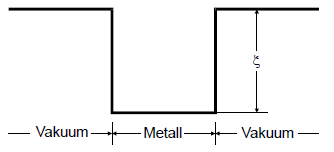
\includegraphics[width = 8cm]{img/Potentialtopf.PNG}
	\caption{Potentialtopfmodell}
	\label{potential_topf}
\end{figure}

Die Elektronen des Kristallgitters unterliegen dem Pauli-Verbot, nach dem nur zwei Elektronen mit entgegengesetztem Spin denselben Zustand mit der Energie $E$ haben k"onnen.
Die Maximalenergie der Elektronen bei T = 0 wird als Grenzenergie $\psi$ bezeichnet.
Die Wahrscheinlichkeit daf"ur, ob ein Zustand mit der Energie $E$ besetzt wird, wird durch die Fermi-Dirac'sche Verteilungsfunktion angegeben:

\begin{equation}
	f(E) = \frac{1}{exp( \frac{E - \psi}{kT} ) + 1} \, .
\end{equation}

Der Verlauf ist in Abb. \ref{fermi} dargestellt.
Die Exponentialfunktion im Nenner "ubertrifft die Zahl 1 bei weitem, wodurch n"aherungsweise gilt:

\begin{equation}
	f(E) \propto exp ( \frac{\psi - E}{kT}) \, .
\end{equation}

\begin{figure}[!h]
	\centering
	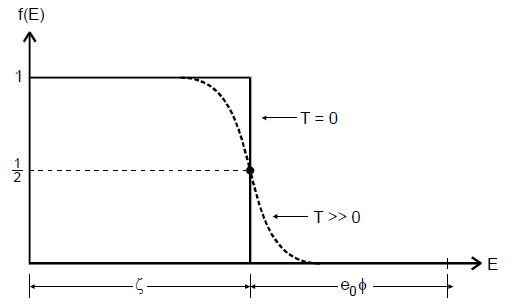
\includegraphics[width = 8cm]{img/Fermi.PNG}
	\caption{Fermi-Dirac'sche Verteilungsfunktion}
	\label{fermi}
\end{figure}

\subsection{Berechnung der S"attigungsstromdichte bei der thermischen Elektronenemission} % (fold)
\label{sub:berechnung_der_s_attigungsstromdichte_bei_der_thermischen_elektronenemission}

F"ur die S"attigungsstromdichte $j_\mathrm{s}(T)$ erh"alt man nach Einf"uhrung eines kartesischen Koordinatensystems die Richardson Gleichung:

\begin{equation}
	j_\mathrm{s}(T) = 4\pi \frac{e_\mathrm{0} m_\mathrm{0} k^2}{h^3} T^2 exp( \frac{-e_\mathrm{0} \Phi}{kT}) \, .
\end{equation}

\subsection{Die Hochvakuum-Diode} % (fold)
\label{sub:die_hochvakuum_diode}

Um Wechselwirkungen mit den Gasmolek"ulen der Luft zu vermeiden, muss die Messung des S"attigungsstroms $j_\mathrm{s}$ im Hochvakuum duchgef"uhrt werden.
Diese ist nach Abb. \ref{diode} aufgebaut.
Durch eine angelegte Heizspannung kann die Gl"uhkathode auf 1000 bis 3000\,K erhitzt werden.

Die austretenden Elektronen werden durch ein elektrisches Feld zur Anode hin beschleunigt. Die Diode wird in der Technik zur Gleichrichtung von Wechselstr"omen benutzt, da die Elektronen nicht in der Lage sind, gegen ein hohes Gegenfeld anzulaufen.

\begin{figure}[!h]
	\centering
	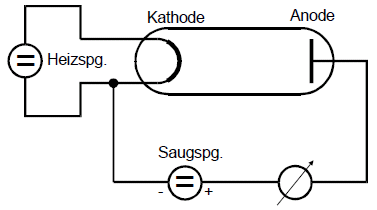
\includegraphics[width = 8cm]{img/Diode.PNG}
	\caption{Beschaltung einer Hochvakuum-Diode}
	\label{diode}
\end{figure}

\subsection{Langmuir-Schottkysche Raumladungsdichte} % (fold)
\label{sub:langmuir_schottkysche_raumladungsdichte}

Der Anodenstrom ist nicht nur von der Kathodentemperatur, sondern auch von der Anodenspannung abh"angig. Dies kommt, da die Geschwindigkeit $v$ der Elektronen nicht konstant ist und so das Ohm'sche Gesetz nicht g"ultig ist.
Daraus folgt, dass die Raumladungsdichte $\rho$ der Elektronen ortsabh"angig ist.
Dies folgt aus der konstanten Kontinuit"atsgleichung

\begin{equation}
	j = - \rho v \, .
\end{equation}

Die Elektronen schirmen also die Feldlinien der Anode vor der Kathode ab.
Um dennoch Zusammenh"ange zwischen Anodenspannung und -strom darstellen zu k"onnen, geht man von der Poisson'schen Gleichung aus:

\begin{equation}
	\Delta V = - \frac{1}{\epsilon_\mathrm{0}} \rho \, .	
\end{equation}

\begin{center}
		\tiny{($\Delta$ = Laplace Operator, V = Potential am Aufpunkt, $\epsilon_\mathrm{0}$ = Dielektrizit"atskonstante des Vakuums)}
\end{center}

Es ergibt sich f"ur den Zusammenhang zwischen Stromdichte $j$ und Anodenspannung $V$:

\begin{equation}
	j = \frac{4}{9} \epsilon_\mathrm{0} \sqrt{2 \frac{e_\mathrm{0}}{m_\mathrm{0}}} \frac{V^\frac{3}{2}}{a^2} \, .
\end{equation}

Dies ist das Langmuir-Schottkysche Raumladungsgesetz und $j$ w"achst mit $V^\frac{3}{2}$.

\begin{figure}[!h]
	\centering
	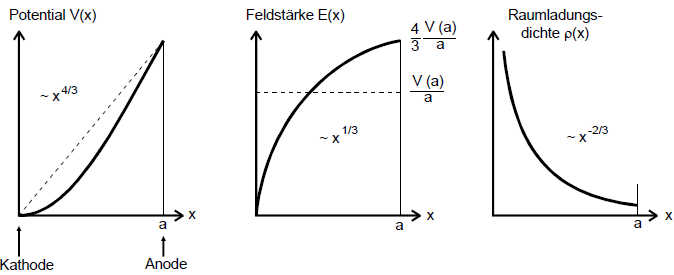
\includegraphics[width = 10cm]{img/schott.PNG}
	\caption{Ortsabh"angigkeit des potentials V, der Feldst"arke E und der Raumladungsdichte $\rho$ im Raumladungsgebiet einer Hochvakuumdiodenkennlinie}
	\label{schott}
\end{figure}

\subsection{Das Anlaufstromgebiet einer Hochvakuumdiode} % (fold)
\label{sub:das_anlaufstromgebiet_einer_hochvakuumdiode}

Bei T > 0 treten endlich viele Elektronen aus dem Material aus. Der Energie"uberschuss dieser Elektronen ist deren kinetische Energie, mit der sie gegen ein geringes Gegenfeld anlaufen k"onnen.
Dieser Strom wird als Anlaufstrom bezeichnet.
Dabei ergibt sich f"ur den Anlaufstrom in Abh"angigkeit vom "au"seren Potential:

\begin{equation}
	j(V) = j_\mathrm{0} \exp{ \left( -\frac{e_\mathrm{0} (\phi_\mathrm{A} + V)}{kT} \right)} = \mathrm{const} \exp{ \left( -\frac{e_\mathrm{0}V}{kT} \right)}\, .
\end{equation}

\subsection{Die Kennlinie der Hochvakuumdiode} % (fold)
\label{sub:die_kennlinie_der_hochvakuumdiode}

Die Kennlinie einer Hochvakuumdiode l"asst sich in das Anlaufstrom-, Raumladungsstrom- und S"attigungsstromgebiet gliedern (Abb. \ref{kennlinie}).
F"ur V < 0 ist im Anlaufstromgebiet ein exponentieller Zusammenhang zu erkennen. F"ur V > 0 ist das Raumladungsstromgebiet proportional zu $\sqrt{V^3}$.
Mit steigendem V strebt der Anodenstrom einem S"attigungswert entgegen.

\begin{figure}[!h]
	\centering
	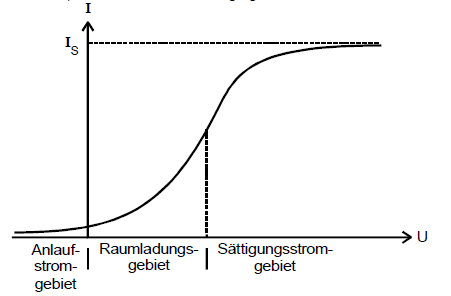
\includegraphics[width = 8cm]{img/kennlinie.PNG}
	\caption{Kennlinie einer Hochvakuumdiode}
	\label{kennlinie}
\end{figure}